\section{Idé}

\begin{frame}{Idé}
\begin{center}
Kan man med \textbf{information} om trafiksignaler og evt. trængsel\\\textbf{spare brændstof} for den enkelte bil\\uden \textbf{nævneværdig påvirkning} af anden trafik?
\end{center}
\includegraphics[width=1\textwidth]{images/figure.png}
\end{frame}

\begin{frame}{Hvad er problemet?}
\textbf{Reducere brændsstofforbug}
\begin{itemize}
\item Miljøhensyn
\item Økonomihensyn
\end{itemize}

Trafiksikkerhed

Maksimering af trafikflow

\vspace{5mm}
\begin{columns}
\begin{column}{0.5\textwidth}
Muligheder
\begin{itemize}
\item Brændstofbesparende kørsel
\item \textbf{Minimere acceleration}
\end{itemize}

\end{column}
\begin{column}{0.5\textwidth}
Forhindinger
\begin{itemize}
\item Anden trafik
\item \textbf{Trafiklys}
\end{itemize}
\end{column}
\end{columns}
\end{frame}

\begin{frame}{Trafiklys}
Minimering af acceleration ved trafiklys
\begin{itemize}
\item Adaptive trafiklys
\item \textbf{Tilpasse bilers hastighed til trafiklysene}
\end{itemize}


\begin{center}
\begin{columns}
\begin{column}{0.5\textwidth}
Fordele
\begin{itemize}
\item Ingen ombygning af eksisterende lys
\item Få invisteringsudgifter 
\item Virker ved lav penetrationsrate
\end{itemize}
\end{column}

\begin{column}{0.5\textwidth}
Ulemper
\begin{itemize}
\item Kræver biler kan aflæse trafiksignaler live
\item Påvirkning af øvrig trafik?
\end{itemize}
\vspace{1cm}
\end{column}
\end{columns}
\end{center}
\end{frame}

\begin{frame}{Hastighedstilpasning}
\begin{itemize}
\item Ét tænkt lyskryds
\item Blå biler: uden systemet \hspace{8mm} Røde biler: med systemet
\end{itemize}
\vspace{3mm}
\includegraphics[width=1\textwidth]{images/eks1.png}
\end{frame}

\begin{frame}{Hastighedstilpasning}
\begin{itemize}
\item Ét tænkt lyskryds
\item Blå biler: uden systemet \hspace{8mm} Røde biler: med systemet
\end{itemize}
\vspace{3mm}
\includegraphics[width=1\textwidth]{images/eks2.png}
\end{frame}

